% \documentclass[linenumbers,floatfix,ApJL,twocolumn]{aastex631}
\documentclass[floatfix,ApJL,twocolumn]{aastex631}

\usepackage{amssymb}
\usepackage{amsmath}
\usepackage{microtype}
\usepackage{url}
\usepackage{xspace}
\usepackage{xcolor}
\usepackage{ifxetex}
\ifxetex
\usepackage{fontspec}
\defaultfontfeatures{Extension = .otf}
\fi
\usepackage{fontawesome}



\setlength{\parindent}{3.0ex}


% Projects:
\newcommand{\project}[1]{\textsf{#1}}

\newcommand{\python}{\project{Python}}
\newcommand{\cython}{\project{Cython}}
\newcommand{\cpp}{\project{C++}}
\newcommand{\jupyter}{\project{Jupyter}}

\newcommand{\exoplanet}{\project{exoplanet}}
\newcommand{\lightkurve}{\project{lightkurve}}
\newcommand{\starry}{\project{starry}}
\newcommand{\theano}{\project{Theano}}
\newcommand{\pymc}{\project{PyMC3}}
\newcommand{\celerite}{\project{celerite}}
\newcommand{\dynesty}{\project{dynesty}}
\newcommand{\astroquery}{\project{astroquery}}
\newcommand{\scipy}{\project{scipy}}
\newcommand{\jupytext}{\project{jupytext}}
\newcommand{\sphinx}{\project{sphinx}}
\newcommand{\jupyterbook}{\project{Jupyter-book}}
\newcommand{\arviz}{\project{ArviZ}}
\newcommand{\nbconvert}{\project{nbconvert}}


\newcommand{\tess}{\project{TESS}}
\newcommand{\kepler}{\project{Kepler}}
\newcommand{\gaia}{\project{Gaia}}

\newcommand{\mast}{\project{MAST}}
\newcommand{\exofop}{\project{ExoFOP}}

\newcommand{\tessAtlas}{\project{TESS Atlas}}

% math
\newcommand{\T}{\ensuremath{\mathrm{T}}}
\newcommand{\dd}{\ensuremath{ \mathrm{d}}}
\newcommand{\unit}[1]{{\ensuremath{ \mathrm{#1}}}}
\newcommand{\bvec}[1]{{\ensuremath{\boldsymbol{#1}}}}


\DeclareMathOperator{\invG}{Inv-\mathnormal{\Gamma}}
\DeclareMathOperator{\N}{\mathcal{N}}
\DeclareMathOperator{\U}{\mathcal{U}}
\DeclareMathOperator{\Un}{\mathcal{U}}
\DeclareMathOperator{\Par}{\mathcal{P}ar}
\DeclareMathOperator{\tmin}{\mathnormal{t_{\rm min}}}
\DeclareMathOperator{\tmax}{\mathnormal{t_{\rm max}}}





%% affiliation shortcuts
\newcommand{\SPA}{School of Physics and Astronomy, Monash University, Clayton VIC 3800, Australia}
\newcommand{\OzGravMonash}{OzGrav: The ARC Centre of Excellence for Gravitational Wave Discovery, Clayton VIC 3800, Australia}
\newcommand{\AMNH}{Department of Astrophysics, American Museum of Natural History, New York, NY 10024, USA}
\newcommand{\CCA}{Center for Computational Astrophysics, Flatiron Institute, New York, NY 10010, USA}
\newcommand{\CUNY}{Graduate Center, City University of New York, 365 5th Avenue, New York, NY 10016, USA}
\newcommand{\BMCC}{Department of Science, BMCC, City University of New York, New York, NY 10007, USA}





\newif\ifdraft
\drafttrue % switch to false in non-draft version (thereby hiding the todos)
\newcommand{\inDraftVersion}[1]{\ifdraft #1\fi} 


% TODOs
\newcommand{\todo}[3]{\inDraftVersion{{\color{#2}\emph{#1}: #3}}}
\newcommand{\dfmtodo}[1]{\todo{DFM}{red}{#1}}
\newcommand{\avi}[1]{\todo{Avi}{red}{#1}}
\newcommand{\alltodo}[1]{\todo{TODO}{red}{#1}}
\newcommand{\citeme}{{\color{red}(citation needed)}}


\newcommand{\red}{\textcolor{red}}
\newcommand{\textuit}[1]{\textit{\underline{#1}}}



%% Numbers
% https://exoplanetarchive.ipac.caltech.edu/docs/counts_detail.html
% https://exoplanetarchive.ipac.caltech.edu/index.html

\newcommand{\numConfirmedPlanets}{5,090} % 
\newcommand{\numCandidatesRemaining}{6,959}

\newcommand{\numTessCandidates}{5,488} % 
\newcommand{\numTessPlanets}{227}
\newcommand{\numAnalysed}{2,833}
\newcommand{\numAnalysedMulti}{151}
\newcommand{\numAnalysedSingle}{68}
\newcommand{\cpuHrs}{$\sim80,000\ \rm{Hrs}$}

%% links

% % % from: https://github.com/rodluger/corTeX
% % % Add code, proof, and animation hyperlinks
% \definecolor{linkcolor}{rgb}{0.1216,0.4667,0.7059}
% \newcommand{\codeicon}{{\color{linkcolor}\faFileCodeO}}

% % % Define the `oscaption` command for open source figure captions
% \newcommand{\oscaption}[2]{\caption{#2 \codelink{#1}}}


% \makeatletter
\newcommand{\github}[1]{\href{#1}{\textcolor{gray}{\faGithubSquare}}}








\shorttitle{The \tess\ Atlas}


\begin{document}

\title{The \tess\ Atlas: an open source catalog of TESS transit fits}

\correspondingauthor{Daniel Foreman-Mackey}
\email{foreman.mackey@gmail.com}

\author[0000-0002-4146-1132{Avi Vajpeyi}
\affiliation{
    School of Physics and Astronomy,
    Monash University,
    Clayton VIC 3800,
    Australia
}
\affiliation{
OzGrav: The ARC Centre of Excellence for Gravitational Wave Discovery,
Clayton VIC 3800,
Australia
}

\author[0000-0002-9328-5652]{Daniel Foreman-Mackey}
\affiliation{
    Center for Computational Astrophysics,
    Flatiron Institute,
    162 5th Ave,
    New York, NY 10010
}












\begin{abstract}
% The Transiting Exoplanet Survey Satellite \tess\ has enabled the discovery of more than five-thousand exoplanet candidates, out of which only a few hundred have been confirmed.
% Exoplanet confirmation requires vetting of candidates by ruling out false positives and follow-up observations and analyses.
We present the \tess\ Atlas, a catalog of candidate exoplanet parameter estimates, from two-minute cadence \tess\  data, to assist the vetting process and follow-up analyses.
This catalog contains posterior estimates for \red{\numAnalysed} \tess\ Objects of Interest, including \red{\numAnalysedMulti} multi-planet candidate systems and \red{\numAnalysedSingle} candidates having data for a single transit.
Our analysis utilises the No-U-Turns Markov chain Monte Carlo algorithm to sample the parameter space with a circular transit model implemented in \exoplanet.
\avi{The \tess\ Atlas esitimates are differnt from the ExoFop}.
We provide posterior samples from our analyses and \jupyter notebooks to reproduce the analyses for each exoplanet candidate.
\end{abstract}

% info on sectors: https://heasarc.gsfc.nasa.gov/docs/tess/sector.html

\keywords{%
  methods: data analysis ---
  methods: statistical ---
  miscellaneous --- catalogs --- surveys
}


\section{Introduction} \label{sec:intro}


% intro version 1
In March 2022, NASA's exoplanet archive surpassed five-thousand confirmed exoplanets, a milestone made possible by data from several observatories, including the Transiting Exoplanet Survey Satellite TESS.
The confirmed exoplanets suggest a diverse population, many of which are within their star's habitable zone.
Furthermore, the search for exoplanets has revealed new information on eclipsing binaries, tidally interacting systems,  comets and exocomets, variable stars, supernovae, and even black holes.
This list of exoplanets may be dramatically increased once the six-thousand exoplanets awaiting validation are processed, more than half of which are candidates detected in TESS data.

% GENERIC TESS INTRO
\textcolor{olive}{[
\textuit{INTRO VERSION 2:}
NASA's Transiting Exoplanet Survey Satellite \tess\ \citep{Ricker:2015:JATIS} concluded its two-year Primary Mission to search for transiting exoplanets orbiting nearby bright stars in July 2020.
During this time, the \tess\ Science Processing Operations Center pipeline SPOC \citep{Jenkins:2016:SPIE}  recorded data with a 2-minute cadence for about $200,000$ pre-selected stars.
Additionally, \tess\ captured full-frame images of its entire field of view over 10- and 30-minute intervals, enabling flux measurements of several million stars.
Between 2, 10 and 30-minute observations, the \tess\ Primary Mission and the ongoing extended missions have identified over \red{$\numTessCandidates$} planet candidates, \red{$\numTessPlanets$} of which have been confirmed as planets \citep{Stassun:2018:AJ, Stassun:2019:AJ, Guerrero:2021:ApJS, Guerrero:2021:AAS}. Furthermore, \tess\ data have revealed new information on eclipsing binaries~\citep{ Guo:2020:MNRAS, Powell:2021:AJ}, tidally interacting systems~\citet{Holoien:2019:ApJ}, comets and exocomets~\citep{Farnham:2019:ApJL, Zieba:2019:A&A, Kuznyetsova:2020:OAP, Woods:2021:PASP, Pavlenko:2021:KPCB}),  variable stars~\citet{Antoci:2019:MNRAS, Handler:2020:NatAs}, supernovae~\cite{Vallely:2021:MNRAS, Fausnaugh:2021:ApJ}, and even black holes~\cite{Jayasinghe:2021:MNRAS}.
]}


The majority of TESS exoplanet candidates were discovered using the photometric transit method.
Unfortunately, systematic effects (e.g. ) and non-planetary astrophysical sources (e.g. stellar granulation and eclipsing binaries) can mimic exoplanet transits.
Hence, to validate these candidates, it is necessary to eliminate false-positives and, if possible, conduct additional observations.

Obtaining higher precision planet parameter estimates will assist us in the vetting process.

More exoplanets will help answer various questionss



\alltodo{As search pipelines improve there will be even more candidates and detections}

\alltodo{para on what having more exoplanet info will do}

\alltodo{talk about inference, detection}
\alltodo{link up with our Bayesian model of noise etc}
In this work we provide a comprehensive catalog of transiting exoplanet posterior estimates for the \red{\numAnalysed} \tess\ Objects of Interest (TOIs) with 2-minute cadence observations from 2018 through 2022.
The posterior distributions provide robust uncertainties for the circular transit model's planet orbital timing parameters, stellar limb darkening, stellar density, mean flux and detector-noise parameters.
The posterior distributions can allow future researchers to study the planet population in detail and assess the reliability of the most Earth-like candidates, \alltodo{list more things that can be done}.

We provide software to reproduce the analyses and results at \atlasUrl.
The website contains one Jupyter notebook for each TOI, demonstrating the end-to-end analysis of a TOI.
The notebooks contain software to download and clean light curve data, implementations of the transit-model and priors for inference, the \pymc sampling stage, and a posterior post-processing step.
The website also documents the method to download our Bayesian parameter inference posterior samples, load them and make various plots.


The remainder of the paper is organised as follows: Section~\ref{sec:method} describes our transit light curve model and the Bayesian framework we use to estimate parameters of exoplanet systems from the observed data.
The analysis results are summarised in Section~\ref{sec:results}.
The catalog, released data, and software to reproduce the results are described in Section~\ref{sec:data} and are available online as supplementary materials (\atlasUrl).
Finally, we provide concluding remarks in Section~\ref{sec:conclusion}.

\section{Method} \label{sec:method}





% Revisiting the Kepler field with TESS: Improved ephemerides using
% TESS 2min data
% https://arxiv.org/pdf/2103.03259.pdf
%NEMESIS: EXOPLANET TRANSIT SURVEY OF NEARBY M-DWARFS IN TESS FFIS I
% https://arxiv.org/pdf/2103.05647.pdf



\alltodo{TOI selection, lightcurve preprocessing, eccentricity posterior postprocessing}



\paragraph{Target selection and setup }



Targets are assigned consecutive TOI IDs. Multi- planet systems are assigned suffixes (.01, .02, etc.) mir- roring the suffixes assigned for the TCE. TEV automat- ically generates a comma-separated values (CSV) file with all necessary parameters for each TOI from the vetted TOI list. Each TOI comes with a table of pa- rameters, a DV summary page, and a full DV report.

TOI parameters reflect the best possible analysis available at the time of vetting.
We use this (same way SPOC uses the initial estimates from the previous stage)


We download the list of TESS objects of interest with two minute cadence data.
We generate a notebook for the TOI -- this notebook contains the software to download the data create the transit model, run parameter estimation and generate plots.

We run a download step -- this uses lightkurve to download data.
We clean the lightkurve by removing outlisers sigma outside a certain value
We then delete data outside the suggested transit times $\pm$ 2 * transit duration.


\paragraph{Transit Model}
We model exoplanet transits as circular (non-interacting) Keplerian orbits around their host star, using \exoplanet~\citep{Foreman-Mackey:2021:JOSS}. Each of the $n$ exoplanets in the system are parameterised by the planets'
\begin{enumerate}
  \item \emph{two reference transit times}, one near the beginning of the observations, $t_{\rm min}[n]$, and one near the end, $t_{\rm max}[n]$, both measured in \tess\ BJD,
  \item \emph{the transit duration} $\tau[n]$, measured in hours,
  \item \emph{the impact parameter} of the orbit, $b[n]$, constrained to be $|b| \le 1$,
  \item \emph{the radius ratio} $k[n]=R_{\rm p}[n] / R_\star$, of the planet radius $R_{\rm p}[n]$ divided by the stellar radius $R_\star$, and
  \item \emph{the approximate transit depth} $\delta[n]$, measured in parts-per-thousand.
\end{enumerate}
In the case that a planet has only a single transit in the data, the second reference time $t_{\rm max}[n]$ is substituted with the planet's orbital period $P[n]$.
The host star's limb darkening profile is approximated using \citet{Kipping:2013:MNRAS}'s quadratic limb darkening law \citep{Claret:2000:A&A, Mandel:2002:ApJL}, parameterised in \starry~\citep{Luger:2019:AJ} by the baseline relative flux of the light curve $f_0$,
the mean stellar density $\rho_\star$,
and two quadratic limb-darkening parameters $u_1, u_2$.
Finally, stellar variability (from e.g. asteroseismic oscillation of the star)  is modelled with a \celerite~\citep{Foreman-Mackey:2017:ascl} Gaussian Process (GP), with a stochastically driven damped harmonic oscillator kernel in linear combination with a jitter term, to capture misspecified error bars and model misspecification.
The GP requires three parameters: the quality factor $Q_{\rm GP}$, the undamped period of the oscillator $\rho_{\rm GP}$, the standard deviation of the process $\sigma_{\rm GP}$.
More details of this transit parameterisation are presented in Appendix~\ref{apdx:model_details}.




\paragraph{Bayesian Inference Framework}

To estimate the posterior distribution on each fitted
parameter, we use a MCMC approach similar to the
procedure outlined in Ford (2005) and implemented i

We use the  noise models, and set the priors on the stellar parameters to be uniform in $T_{\rm eff}$ and uniform in the mass-radius relation with Gaussian priors on the parallax, stellar radius, and stellar density from the Gaia DR2 catalog.  For the transiting exoplanet, we set uniform priors on the period, mid-transit time, and transit duration.  We set uniform priors on the planet-to-star radius ratio and log($e$), and set uniform priors on the stellar inclination and the argument of periastron.  We set uniform priors on the log($\sigma_{\rm wn}$) and log($\sigma_{\rm cn}$) parameters.  For the posterior sampling, we use the NUTS| sampler, and run the sampler for 5000 steps with a burn-in of 1000 steps.  We use the

To define our prior distributions for the orbital period, we use a log-normal distribution with a mean value set to the TLS-detected period, and a
standard deviation set to the TLS period error. For the prior
distributions used for the mid-transit time, we use a normal
distribution, with the mean value set to the TLS transit time,
and the standard deviation set to the TLS transit duration. For
our prior distribution of planet-to-star radius ratio, we use a
% uniform distribution ranging from 0.01 to RP/RS + σRP/RS.
% To calculate the uncertainty for the planet-to-star radius ratio,
% σRP/RS, we query the TIC to obtain the stellar radius a

n
Rowe et al. (2014). Our algorithm uses a Gibbs sampler to shuffle the value of parameters for each step of
the MCMC procedure with a control set of parameters
to approximate the scale and orientation for the jumping
distribution of correlated parameters as outlined in Gregory (2011). Our method allows the MCMC approach to
efficiently sample parameter space even with highly correlated model parameters. We generated Markov Chains
with lengths of 100 000 for each PC. T




In this study we use a limb-darkened, circular, Keplerian transit model, as described in Section~\ref{sec:model}.
The likelihood function

The standard likelihood function used to analyse gravitational-wave transients is defined in, e.g. Finn (1992) and Romano \& Cornish (2017), where both the data and the model are expressed in the frequency domain. This likelihood has stationary Gaussian noise, which is a good approximation in most cases (e.g. Berry et al. 2015; Abbott et al. 2017a, 2019a) unless one of the instruments is affected by a glitch (Pankow et al. 2018; Powell 2018). We assume the noise power spectral density (PSD) is independent of the model parameters and therefore ignore the normalization term, yielding



This was achieved
by cutting out short-duration windows around each expected transit
(2 days either side of the transit, unless the planet period was $\geq2$
days) and finding the best-fit of the transit model within that interval.
For consistency only the transit time and mean flux were allowed to
vary in this step, both of which were set as wide Normal distributions
centred on the values found from the chi-squared fit. To begin with,
three iterations of exoplanet’s inbuilt optimize routine were used
to hone in on the true transit times, before PyMC3 (Salvatier et al.
2016) was used to fit the final planet model to each individual Kepler
transit. This was achieved using a two-chain Markov-Chain Monte
Carlo (MCMC) analysis with 1000 tuning steps and 5000 draws
for each object. Longer chains were tested briefly, but increasing
the length further for these relatively simple fits was not found to
change the results significantly. Convergence was assessed using
the Gelman-Rubin statistic and a visual examination of the trace.
Statistically significant values for the final time and error for each
individual transit were then found from the mean and standard
deviation of the MCMC trace.

%
%
%GPs are stochastic models consisting of a mean function
%$\mu_\vec{\theta}(\vec{x})$ and a covariance, autocorrelation, or ``kernel''
%function $K$ parameterized by
%$\vec{\theta}$ and $\vec{\alpha}$ respectively.
%Under this model, the log-likelihood function $\mathcal{L}
%(\vec{\theta},\,\vec{\alpha})$ with a dataset
%
%\begin{align}\eqlabel{gp-likelihood}
%\ln \mathcal{L} (\vec{\theta},\,\vec{\alpha})
%&= -\frac{1}{2} r(\vec{\theta})^{T}\, K(\vec{\alpha})^{-1}\, r(\vec{\theta}) \nonumber \\
%   -\frac{1}{2} \log \det K(\vec{\alpha})
%
%\end{align}



\paragraph{Website generation}
Generate webpages using notebooks



\section{Results}\label{sec:results}


To provide context for our planet candidates in regard to
planet demographics and the radius valley, we display our
planet candidates in the planet radius–period space, and compare them with nearby candidates from the TOI and DIAmante catalogs, together with additional confirmed transiting planets observed in





\subsection{Systems with multiple planets}
Some words about these systems

\subsection{Planets with data for one transit}
Some stuff about single transit systems


\section{Data and software availability}\label{sec:data}

he DV module produces a one-page PDF summary report for each TCE, a PDF full report, and a PDF mini report for each target. The full report for each target with TCEs includes the results of all the tests along with diagnostic figures and run time warnings and errors. The mini-report for each target with TCEs combines the one-page summary along with the most informative diagnostic tests and graphics from the full report. An example one-page summary is shown in Figure 2. The DV module also produces a FITS file of the time series it analyzes as well as those presented in the diagnostic plots, and an XML file with numerical model fit and diagnostic test results (Tenenbaum  Jenkins 2018).

We provide software to reproduce the analyses and results at \atlasUrl.
The website contains one Jupyter notebook for each TOI, demonstrating the end-to-end analysis of a TOI.
The notebooks contain software to download and clean light curve data, implementations of the transit-model and priors for inference, the \pymc sampling stage, and a posterior post-processing step.
The website also documents the method to download our Bayesian parameter inference posterior samples, load them and make various plots.

\section{Discussion}\label{sec:conclusion}
We present for the first time a catalog of Bayesian posterior samples for the 2-minute cadence TOIs from 2018-2022.
Some words about results.
Some stuff about difficulty sampling grazing systems.
Errors when SPOC estimates are off.
We expect the remainder of the \tess\ extended mission will complete by September 2023, at which point an updated catalog will be produced.

Vetters can identify false positive TCEs by a few tell- tale signs: a visible secondary eclipse which cannot phys- ically be planetary in nature; a mismatch between odd and even transit depths caused by a stellar binary at twice the indicated period; a shift of the centroid to another nearby star; and increasing transit depth with aperture size, indicative that a signal is from an object nearby on the sky and not the suspected target star.

Lots of manual vetting requiured to promote TCE to TOI. In the future this work can help with that process.


%%%%%%%%%%%%%%%%%%%%

\begin{figure}
  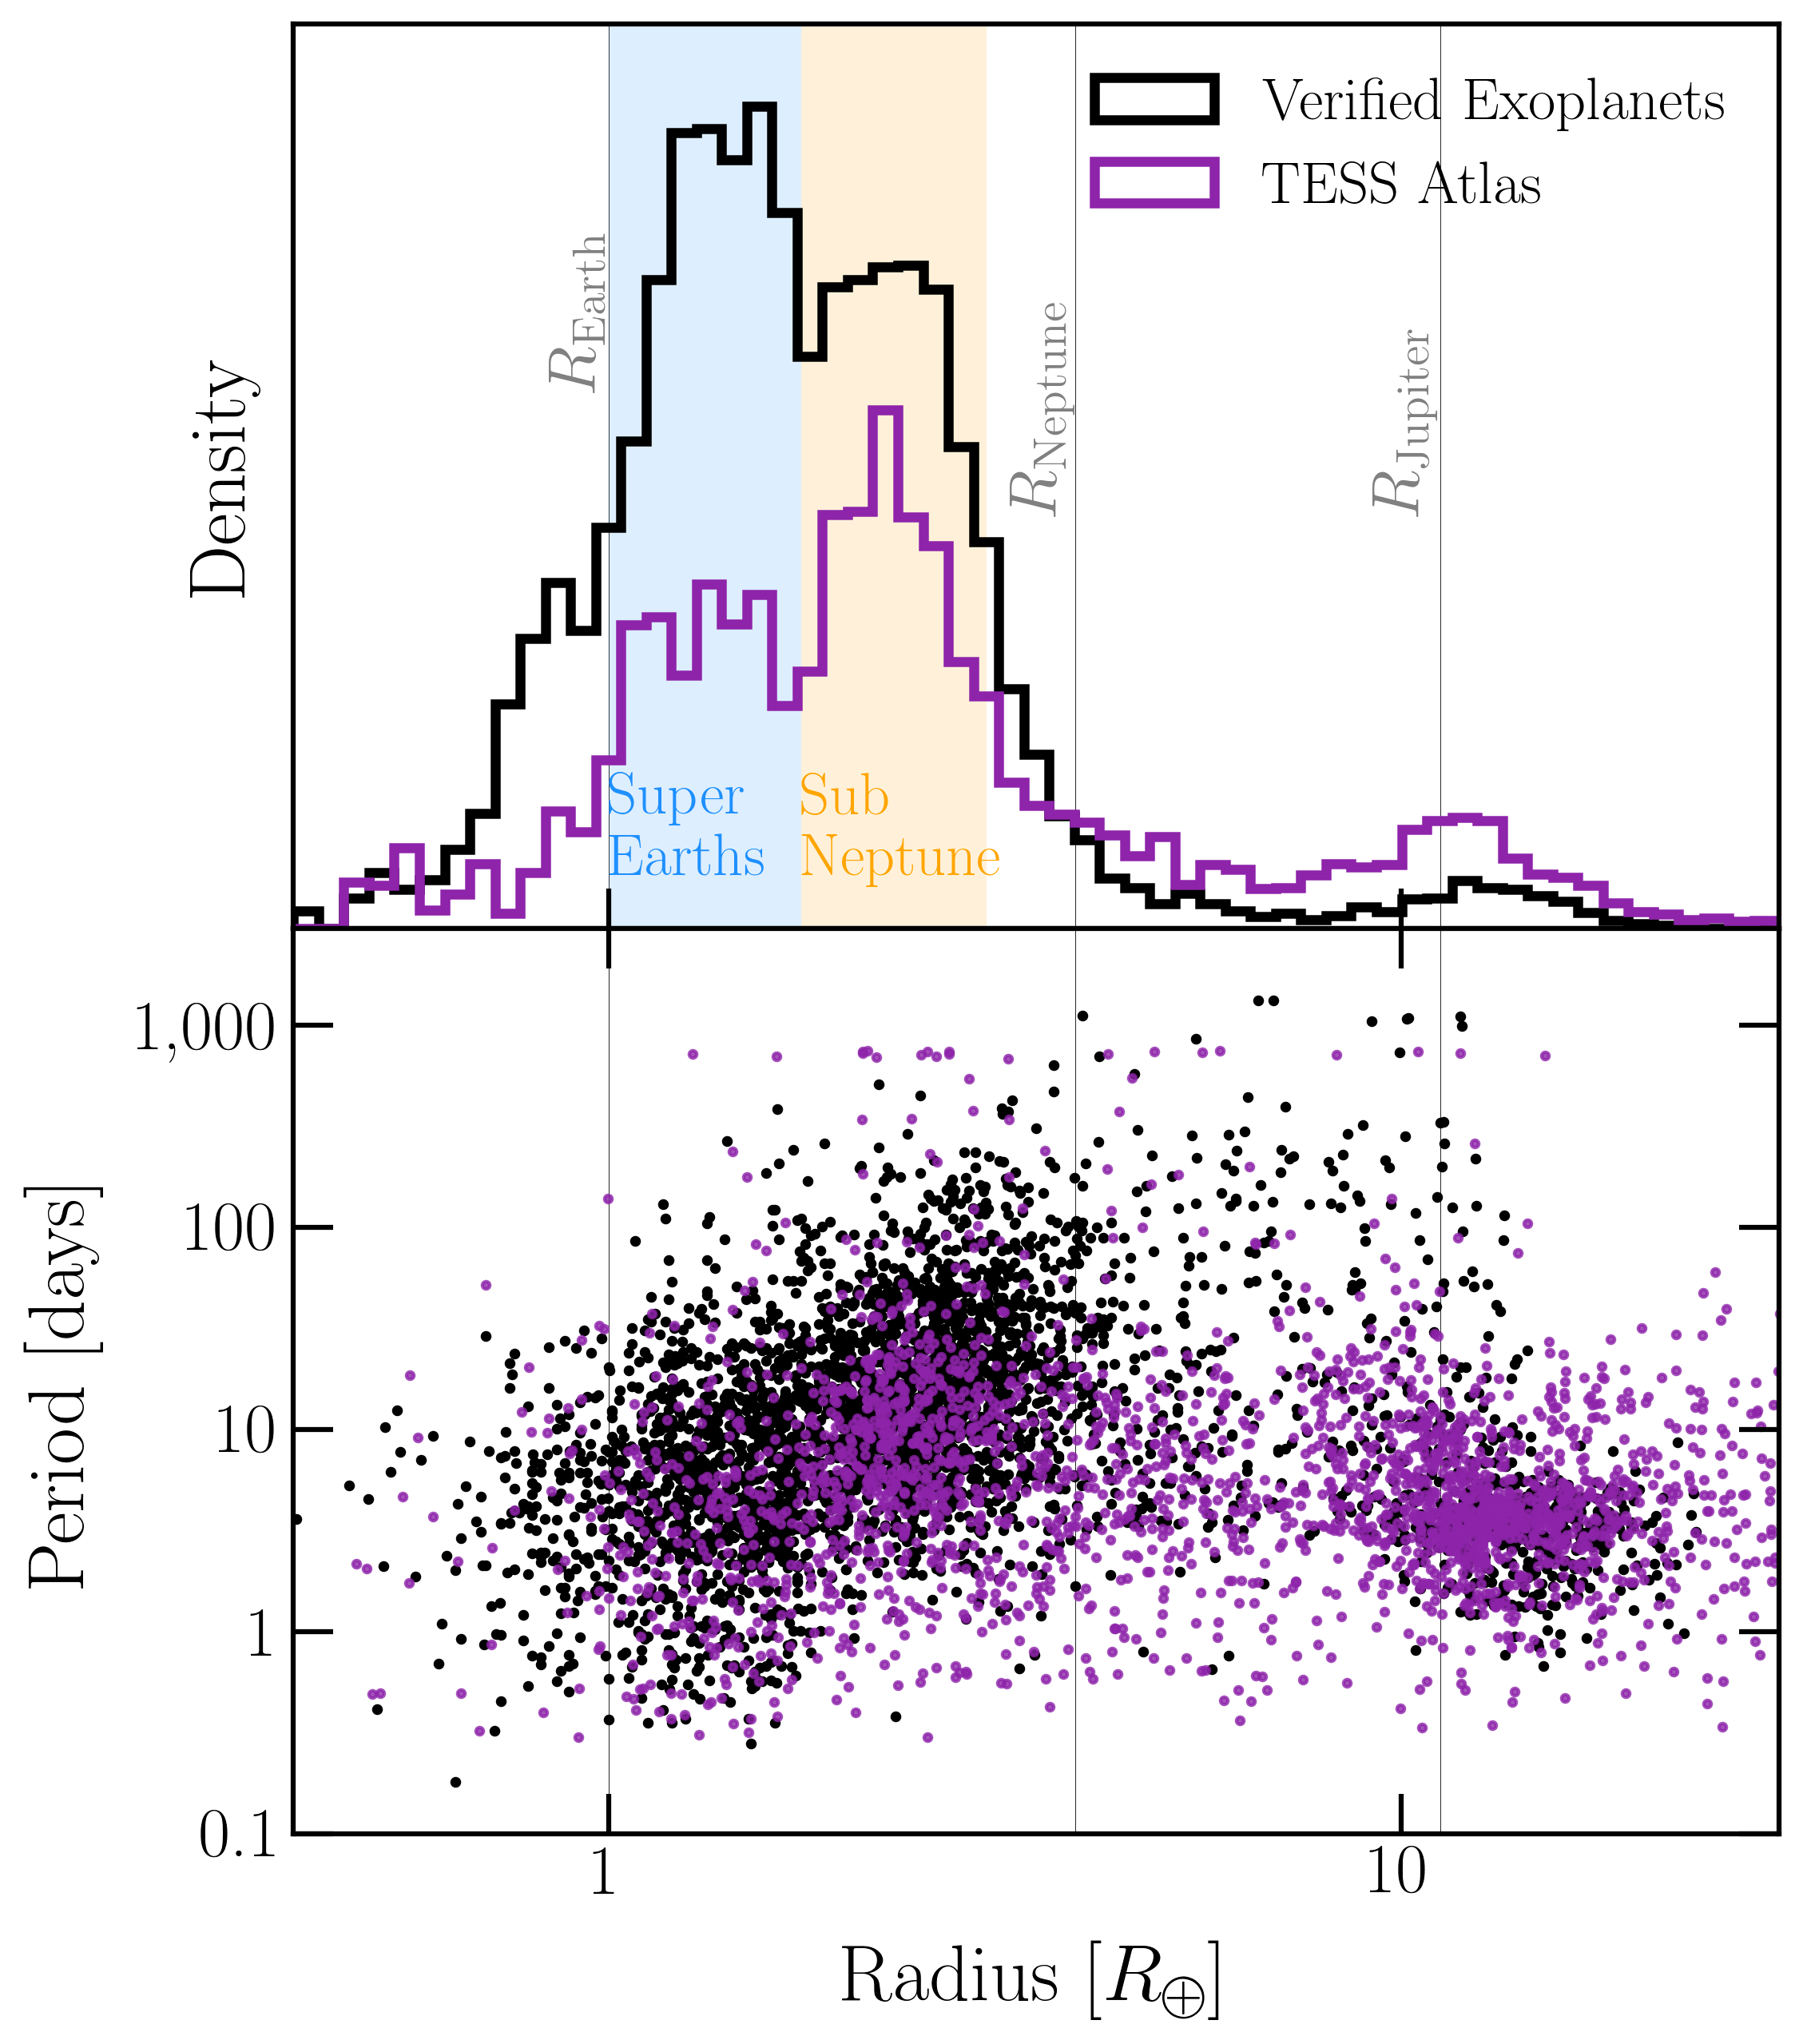
\includegraphics[width=\linewidth]{figures/radius_period_plot.png}
  \caption{\textbf{Main caption:} stuff }
  \label{fig:}
\end{figure}


\begin{figure}
  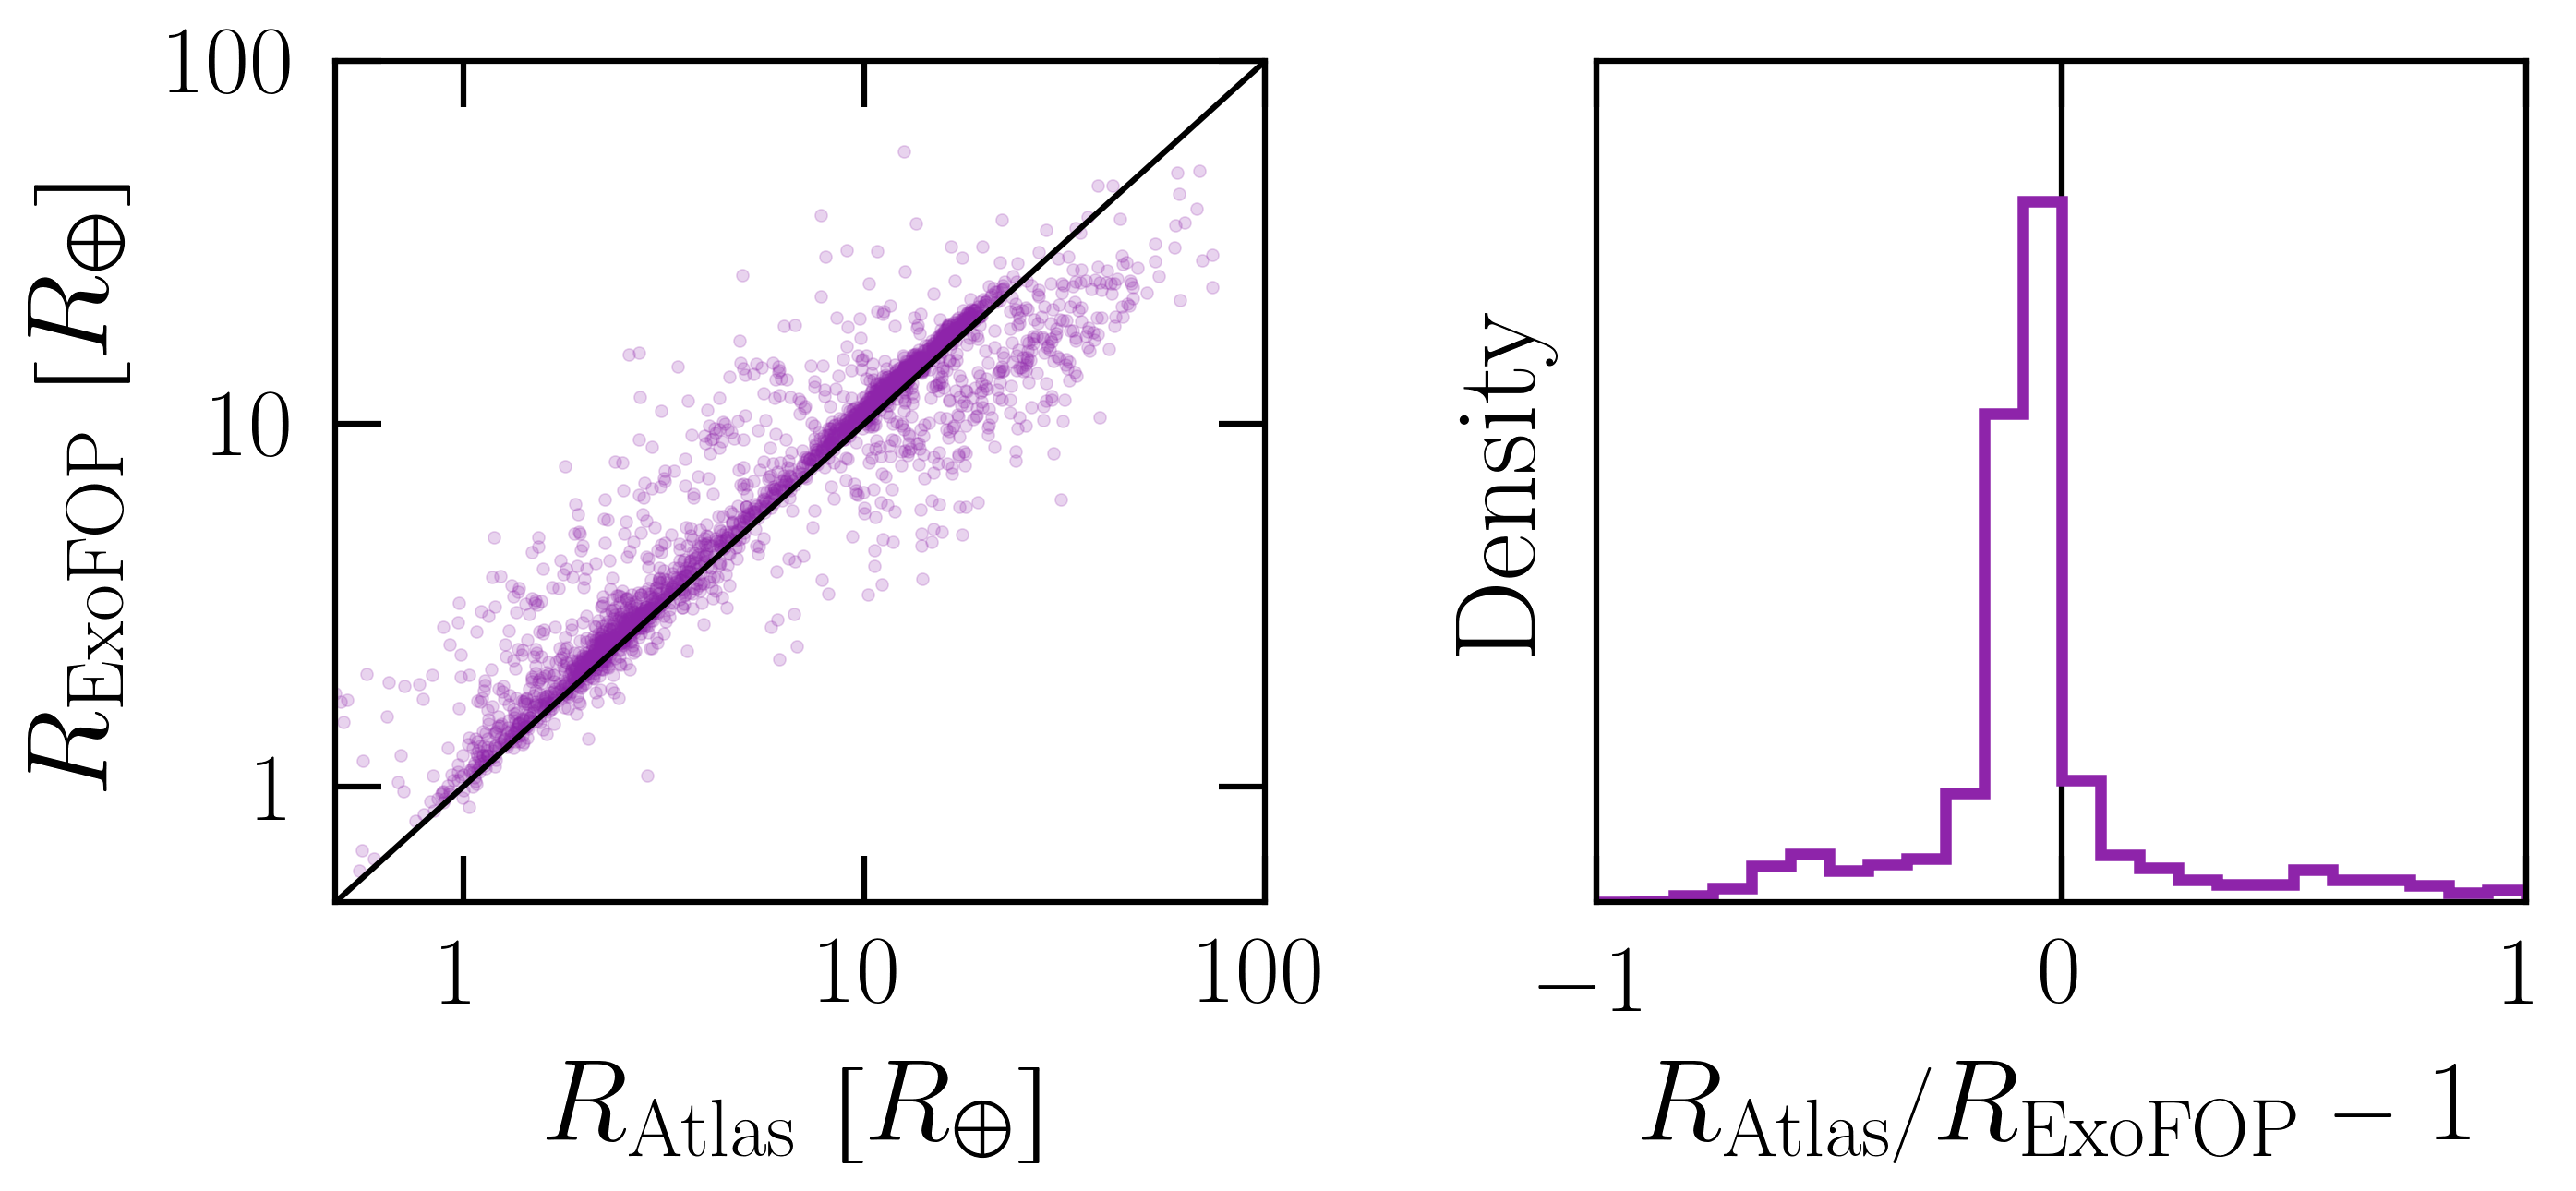
\includegraphics[width=\linewidth]{figures/radius_error.png}
  \caption{\textbf{Main caption:} stuff }
  \label{fig:}
\end{figure}

\begin{figure}
    \gridline{\fig{figures/phase_plot_TOI174_1.png}{0.95\linewidth}{}}
    \gridline{\fig{figures/phase_plot_TOI174_4.png}{0.95\linewidth}{}}
    \caption{Inverted pyramid figure of six individual }
    \label{fig:}
\end{figure}




\section*{Acknowledgments}{

We would like to thank xyz.
Ozgrav, Flatiron, NECTAR, ADACS, David Liptai
Work was started during `online.tess.science`

This work has made use of the TIC through the TESS Science Office’s target selection working group (architects K. Stassun, J. Pepper, N. De Lee, M. Paegert, R. Oelkers).

This research has made use of the NASA Exoplanet Archive, which is operated by the California Institute of Technology, under contract with the National Aeronautics and Space Administration under the Exoplanet Exploration Program.

This work made use of the \tess\ catalog on ExoFOP

Total compute time for this work \red{\cpuHrs} \alltodo{get more accurate compute time (this is an overestimate)}. CO$_2$ emission amount for this work would be XX, however as OzStar uses wind energy this has a negligible carbon footprint.

}

\vspace{5mm}
\facilities{\tess, \gaia, \kepler, Exoplanet Archive, etc.}

\software{
astropy \citep{Astropy-Collaboration:2013,Astropy-Collaboration:2018},
exoplanet,
lightkurve,
starry,
celerite2,
pymc3,
numpy,
scipy,
pandas,
matplotlib,
corner,
sphinx,
}


% ADS bibliography link
% https://ui.adsabs.harvard.edu/user/libraries/_DyLS4HbTY-eJIMBiFUdxw
\bibliography{atlas}{}
\bibliographystyle{aasjournal}

%%%%%%%%%%%%%%%%%%%%%%%%%%%%%%%%%%%%%%%%%%%%
\appendix

\section{Transit model parameterisation details}\label{apdx:model_details}

\paragraph{Transit depth}
The small planet approximation of the transit depth, $\delta=k^2$, is useful as it is directly invertible (conditioned on the limb darkening parameters and impact parameter).
However, the parameterisation restricts the model to non-grazing transits with impact parameter $|b| \le 1$.
Accepting this restriction, we can compute the approximate transit depth for a limb darkened light curve by assuming that the intensity of the star is uniform under the disk of the planet.
For quadratic limb darkening, the intensity profile is
\begin{equation}
  I(r) = 1 - u_1\,[1 - \mu(r)] - u_2\,[1 - \mu(r)]^2
\end{equation}
where $\mu(r) = \sqrt{1 - r^2}$.
The ratio of the occulted flux to the total stellar flux when the transit is deepest ($r = b$) is \citep[the same results are discussed by][]{Mandel:2002,Csizmadia:2013, Agol:2020:AJ}
\begin{eqnarray}
  \delta &\approx& \frac{\int_0^k\,2\,\pi\,r\,I(b)\dd r}{\int_0^1\,2\,\pi\,r\,I(r)\dd r} \nonumber\\
  &=& \frac{k^2\,\left(1 - u_1\,[1 - \mu(b)] - u_2\,[1 - \mu(b)]^2\right)}{1 - u_1/3 - u_2/6}\quad.
\end{eqnarray}
Therefore, since $k$ must be positive, we have a one-to-one transformation between $\delta$ and $k$ conditioned on impact parameter $|b| \le 1$ and the limb darkening coefficients.
It is also important to include the Jacobian factor so that fitting in $\delta$ doesn't introduce a strange prior on $r$.
In this case, the relevant factor is
\begin{equation}
  \left|\frac{\dd k}{\dd \delta}\right| = \left|\frac{1 - u_1/3 - u_2/6}{2\,k\,\left(1 - u_1\,[1 - \mu(b)] - u_2\,[1 - \mu(b)]^2\right)}\right| \quad.
\end{equation}


\paragraph{Transit times}
To expedite the analysis, we assume that the \exofop\ period and phase of the orbit are sufficiently accurate to fit only the data nearby the anticipated transit times (with some buffer, $\pm2\tau$) and disregard the remaining data.
This implies that the number of periods $N_P$ in the TESS observational baseline is exact and the transits must occur within the data cutouts.
This can be difficult to enforce---especially for low signal-to-noise transits.
A good approximation can be achieved by fitting for two reference transit times, $t_{\rm min}$ and $t_{\rm max}$, with a fixed number of periods, $N_P$, between them, instead of a single reference time and the period.
Then the implied period can be computed as $P = (t_{\rm max} - t_{\rm min}) / N_P$.
Importantly this does not change the prior on $P$ and $t_0$ since the Jacobian is a constant $1/N_P$.


\paragraph{Transit duration}
The transit duration $\tau$ is better constrained than the orbit's semi-major axis, $a$ the so it can be better as a fit parameter.
For a circular orbit, the transit duration is \citep{Winn:2010}
\begin{equation}
  \tau = \frac{P}{\pi}\,\sin^{-1}\left( \frac{\sqrt{(1 + k^2) - b^2}}{a\,\sin i} \right) \quad.
\end{equation}
Rearranging this, we find
\begin{equation}
  a^2\,\sin^2 i\,\sin^2\left(\frac{\pi\,\tau}{P}\right) = (1 + k^2) - b^2 \quad.
\end{equation}
Then, using the fact that $\cos^2 i = b^2 / a^2$, we find
\begin{equation}
  a^2 = \frac{(1 + k)^2 - b^2\,\cos^2\phi}{\sin^2\phi}
\end{equation}
for $\phi = \pi\,\tau / P$.
And the Jacobian is
\begin{eqnarray}
  \frac{\dd a}{\dd \tau} &=& \frac{\pi\,\cos \phi}{a\,P\,\sin^3 \phi}\,\left[b^2 - (1 + k)^2\right] \quad.
\end{eqnarray}

Finally, from the period and semi-major axis, we can compute the implied stellar density (under this assumption of a circular orbit)
\begin{equation}
  \rho_\mathrm{circ} = \frac{3\,\pi\,a^3}{G\,P^2} \quad.
\end{equation}
It is important to note that this is not necessarily the same as the actual stellar density and that, in a multi-planet system, this implied density won't be the same for each planet \citep[see, for example,][]{Dawson:2012, Kipping:2012}.



\end{document}
